In \autoref{abb:ProdukteRT} werden verwendbare Dienste von \ac{AWS}, gemeinsam mit ihren jeweiligen Einsatzgebieten gezeigt. In diesem Abschnitt soll besonders auf die Dienste zum Datenstreaming und zur Datenverarbeitung eingegangen werden. Gezeigt werden jedoch auch Dienste für -Speicherung, -Visualisierung und Machine Learning, da diese komplementär oder mit den prozessierten Daten verwendet werden können.
\begin{figure}[H]
\centering
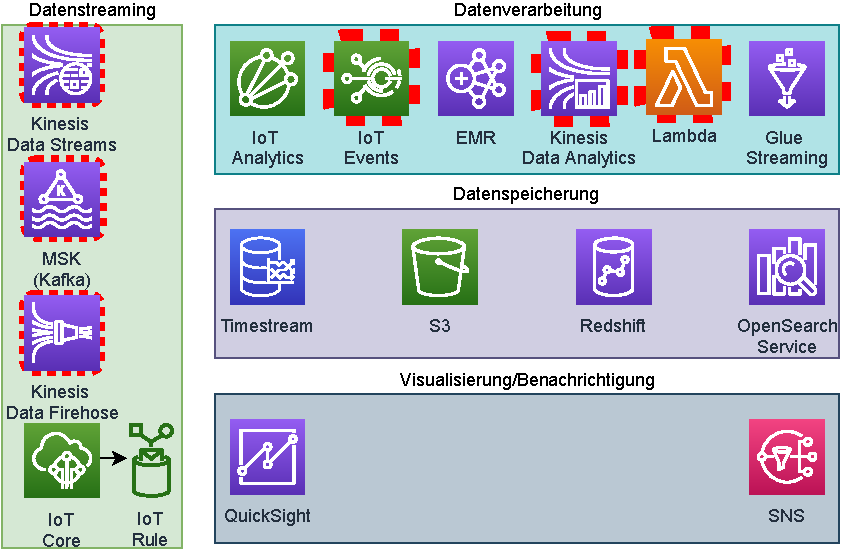
\includegraphics[width=\textwidth]{graphics/Overview-Realtime.pdf}
\caption{Einsetzbare Produkte im Bereich Echtzeitverarbeitung}
\label{abb:ProdukteRT}
\end{figure}


Innerhalb des \ac{IoT} Core Brokers ist es möglich, Regeln zu definieren, die einzelne Nachrichten aus Topics in andere Dienste weiterzuleiten. Dazu müssen besagte Nachrichten selektiert werden, was mittels eines SQL Dialekts möglich ist. Eine beispielhafte Selektion könnte folgendermaßen aussehen: 


\begin{figure}[H]
\centering
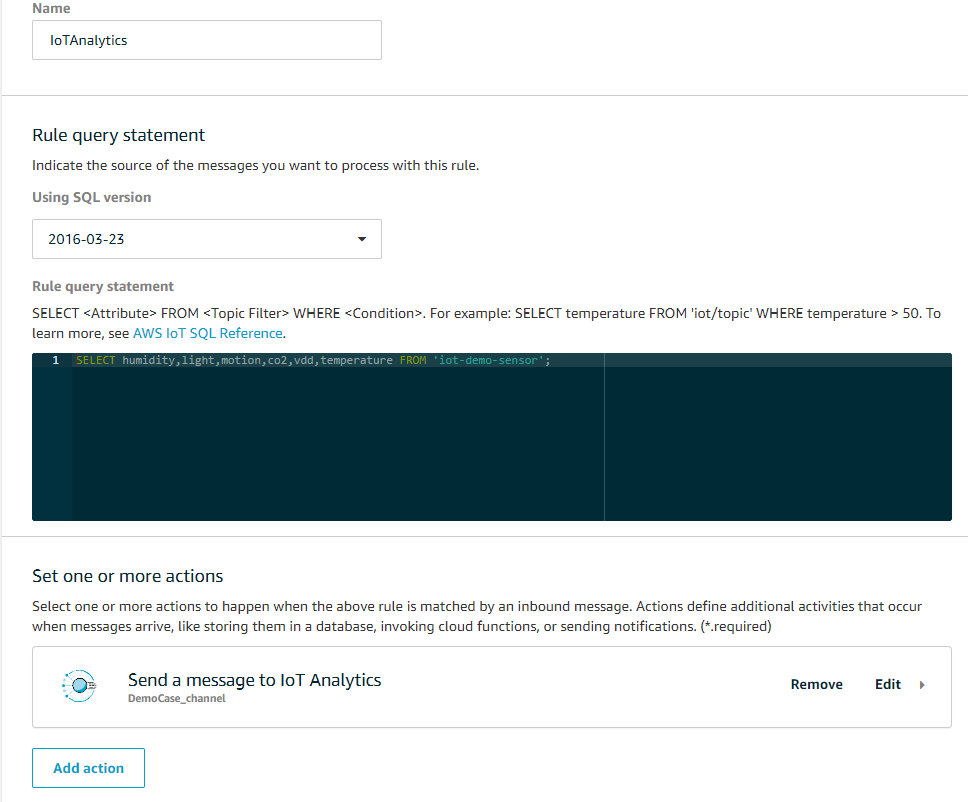
\includegraphics[width=\textwidth]{graphics/IoT-Rules-console.png}
\caption{Einstellung einer neuen Regel zur Weiterleitung an IoT Analytics}
\label{abb:IoTRulesExample}
\end{figure}

In \autoref{abb:IoTRulesExample} ist die Erstellung einer Weiterleitungsregel mit folgendem SQL Code zu sehen:
\lstset{language=SQL} 
\begin{lstlisting}
SELECT humidity,light,motion,co2,vdd,temperature 
FROM 'iot-demo-sensor'
\end{lstlisting}
Die Nachrichten aus dem Topic iot-demo-sensor werden dabei beispielhaft an IoT Analytics weitergeleitet.

\begin{table}[H]
\centering
\begin{tabular}{|l|l|l|}
\hline
\rowcolor[HTML]{ECF4FF} 
Begründung & Kriterium & Bewertung \\ \hline
Einsatz von Code & Robustness and fault tolerance & 8 \\ \hline
Einsatz von Code, statische Analyse & Ad hoc queries & 0 \\ \hline
Anzahl der AWS-Dienste\textless{}5 & Integration mit AWS & 1 \\ \hline
Anzahl der AWS-Dienste=0 & Integration mit AWS & 0 \\ \hline
AWS-properitär & Übertragbarkeit & 0 \\ \hline
\end{tabular}
\caption{Spezielle Einstufungen einzelner Produktbesonderheiten}
\label{tab:einstufungen}
\end{table}



\subsection{AWS IoT Events}
Im Rahmen der \AWSIOT Produktfamilie gibt es neben dem bereits angesprochenen \AWSIOT Analytics ebenfalls \AWSIOT Events.  
Der Dienst dient nach Angaben von Amazon der Konfiguration von \enquote{If-Then-Else} Regeln, mit denen Ereignisse (also Events) erkannt und verarbeitet werden sollen, indem Aktionen ausgelöst werden.\footcite[Vgl.][]{AmazonWebServicesInc..o.J.b} Die Abläufe können dabei, ähnlich wie bei Node-Red graphisch konfiguriert werden. 
\begin{figure}[H]
\centering
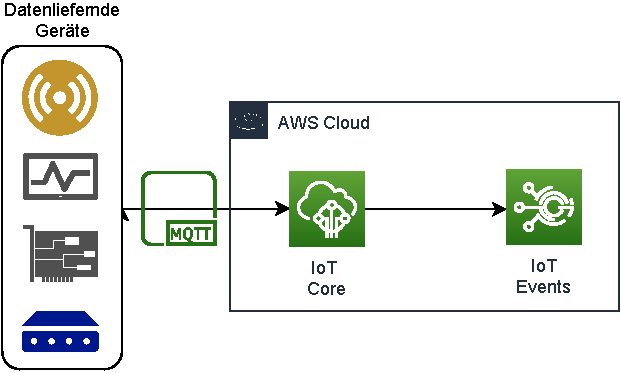
\includegraphics[width=0.8\textwidth]{graphics/IoT-Events-general.pdf}
\caption{Grobarchitektur des Ablaufes für IoT Events}
\label{abb:GrobArchitekturIoTEvents}
\end{figure}

\AWSIOT Events basiert auf abgebildeten Zuständen, die basierend auf ihren Übergängen Aktionen auslösen. \autoref{abb:BeispielIoTEvents} zeigt 3 beispielhaft 3 definierte Zustandsübergänge in der Weboberfläche von \AWSIOT Events. Jeder Kreis, welcher einen Zustand simbolisiert, hat 3 eigene Ereignisse, nämlich OnEnter, OnInput und OnExit. Zusätzlich sind Zustände mit Zustandsübergangspfeilen verbunden, welche basierend auf einer Ausführungskondition ausgelöst werden. Eine solche Ausführungskondition (auch Trigger genannt) wäre beispielsweise
\begin{lstlisting}
$input.Input1.value > $variable.threshold
\end{lstlisting}
\begin{figure}[H]
\centering
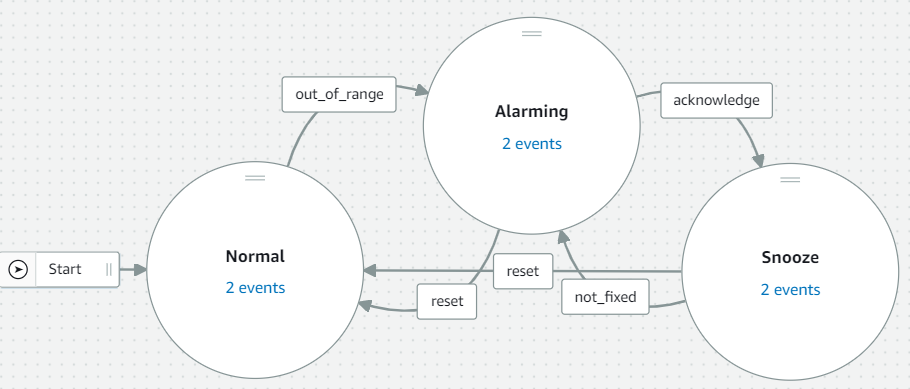
\includegraphics[width=\textwidth]{graphics/IoT-Events-Demo.png}
\caption{Beispiel IoT Events}
\label{abb:BeispielIoTEvents}
\end{figure}

\produktbewertung{AWS~IoT~Events}{9,10,9,8,7,3,5,0,0,1,0,47}
\autoref{tab:bewertungsmatrix-AWS~IoT~Events}

\subsection{Amazon Kinesis}
Amazon Kinesis ist im Gegensatz zu \AWSIOT Analytics nicht allein auf die Analyse von \ac{IoT} Daten spezialisiert. Kinesis eignet sich vielmehr für generelle Analysen von allerlei Streamingdaten. Zusätzlich ist Amazon Kinesis älter als \AWSIOT Analytics und bildet die technische Grundlage für die Verarbeitung \AWSIOT Events.\footcite[Vgl.][]{Pogosova.28.05.2020} Kinesis garantiert zusätzlich, dass Daten in 70 Milisekunden verfügbar sind.

\begin{figure}[H]
\centering
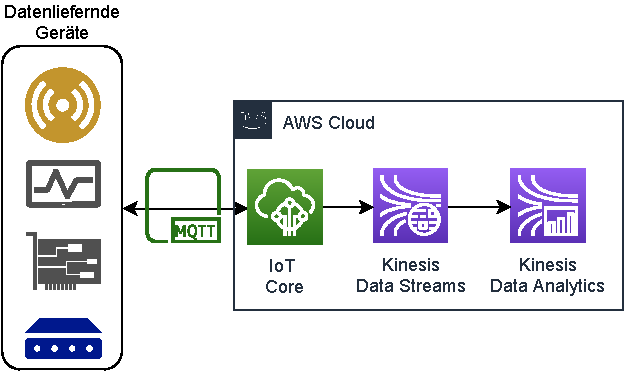
\includegraphics[width=0.8\textwidth]{graphics/Kinesis-Analytics-general.pdf}
\caption{Grobarchitektur des Ablaufes für Kinesis Analytics}
\label{abb:GrobArchitekturKinesisAnalytics}
\end{figure}
In \autoref{abb:GrobArchitekturKinesisAnalytics} ist das Zusammenspiel der Dienste aus der Kinesis Familie mit anderen Diensten dargestellt. Angenommen werden dabei die in \autoref{chap:rahmendatenverarbeitung} erläuterten Rahmenbedingungen, weshalb \ac{IoT} Core als Message Broker eingesetzt ist. Wie in der in \autoref{productselection:iotanalytics} beschriebenen Architektur, muss auch hier für die Datenverarbeitung eine Regel im \ac{IoT} Core Broker angelegt werden, um relevante Nachrichten an Kinesis Data Streams weiterzuleiten.\footcite[Vgl.][]{AmazonWebServicesInc..o.J.}

\begin{figure}[H]
\centering
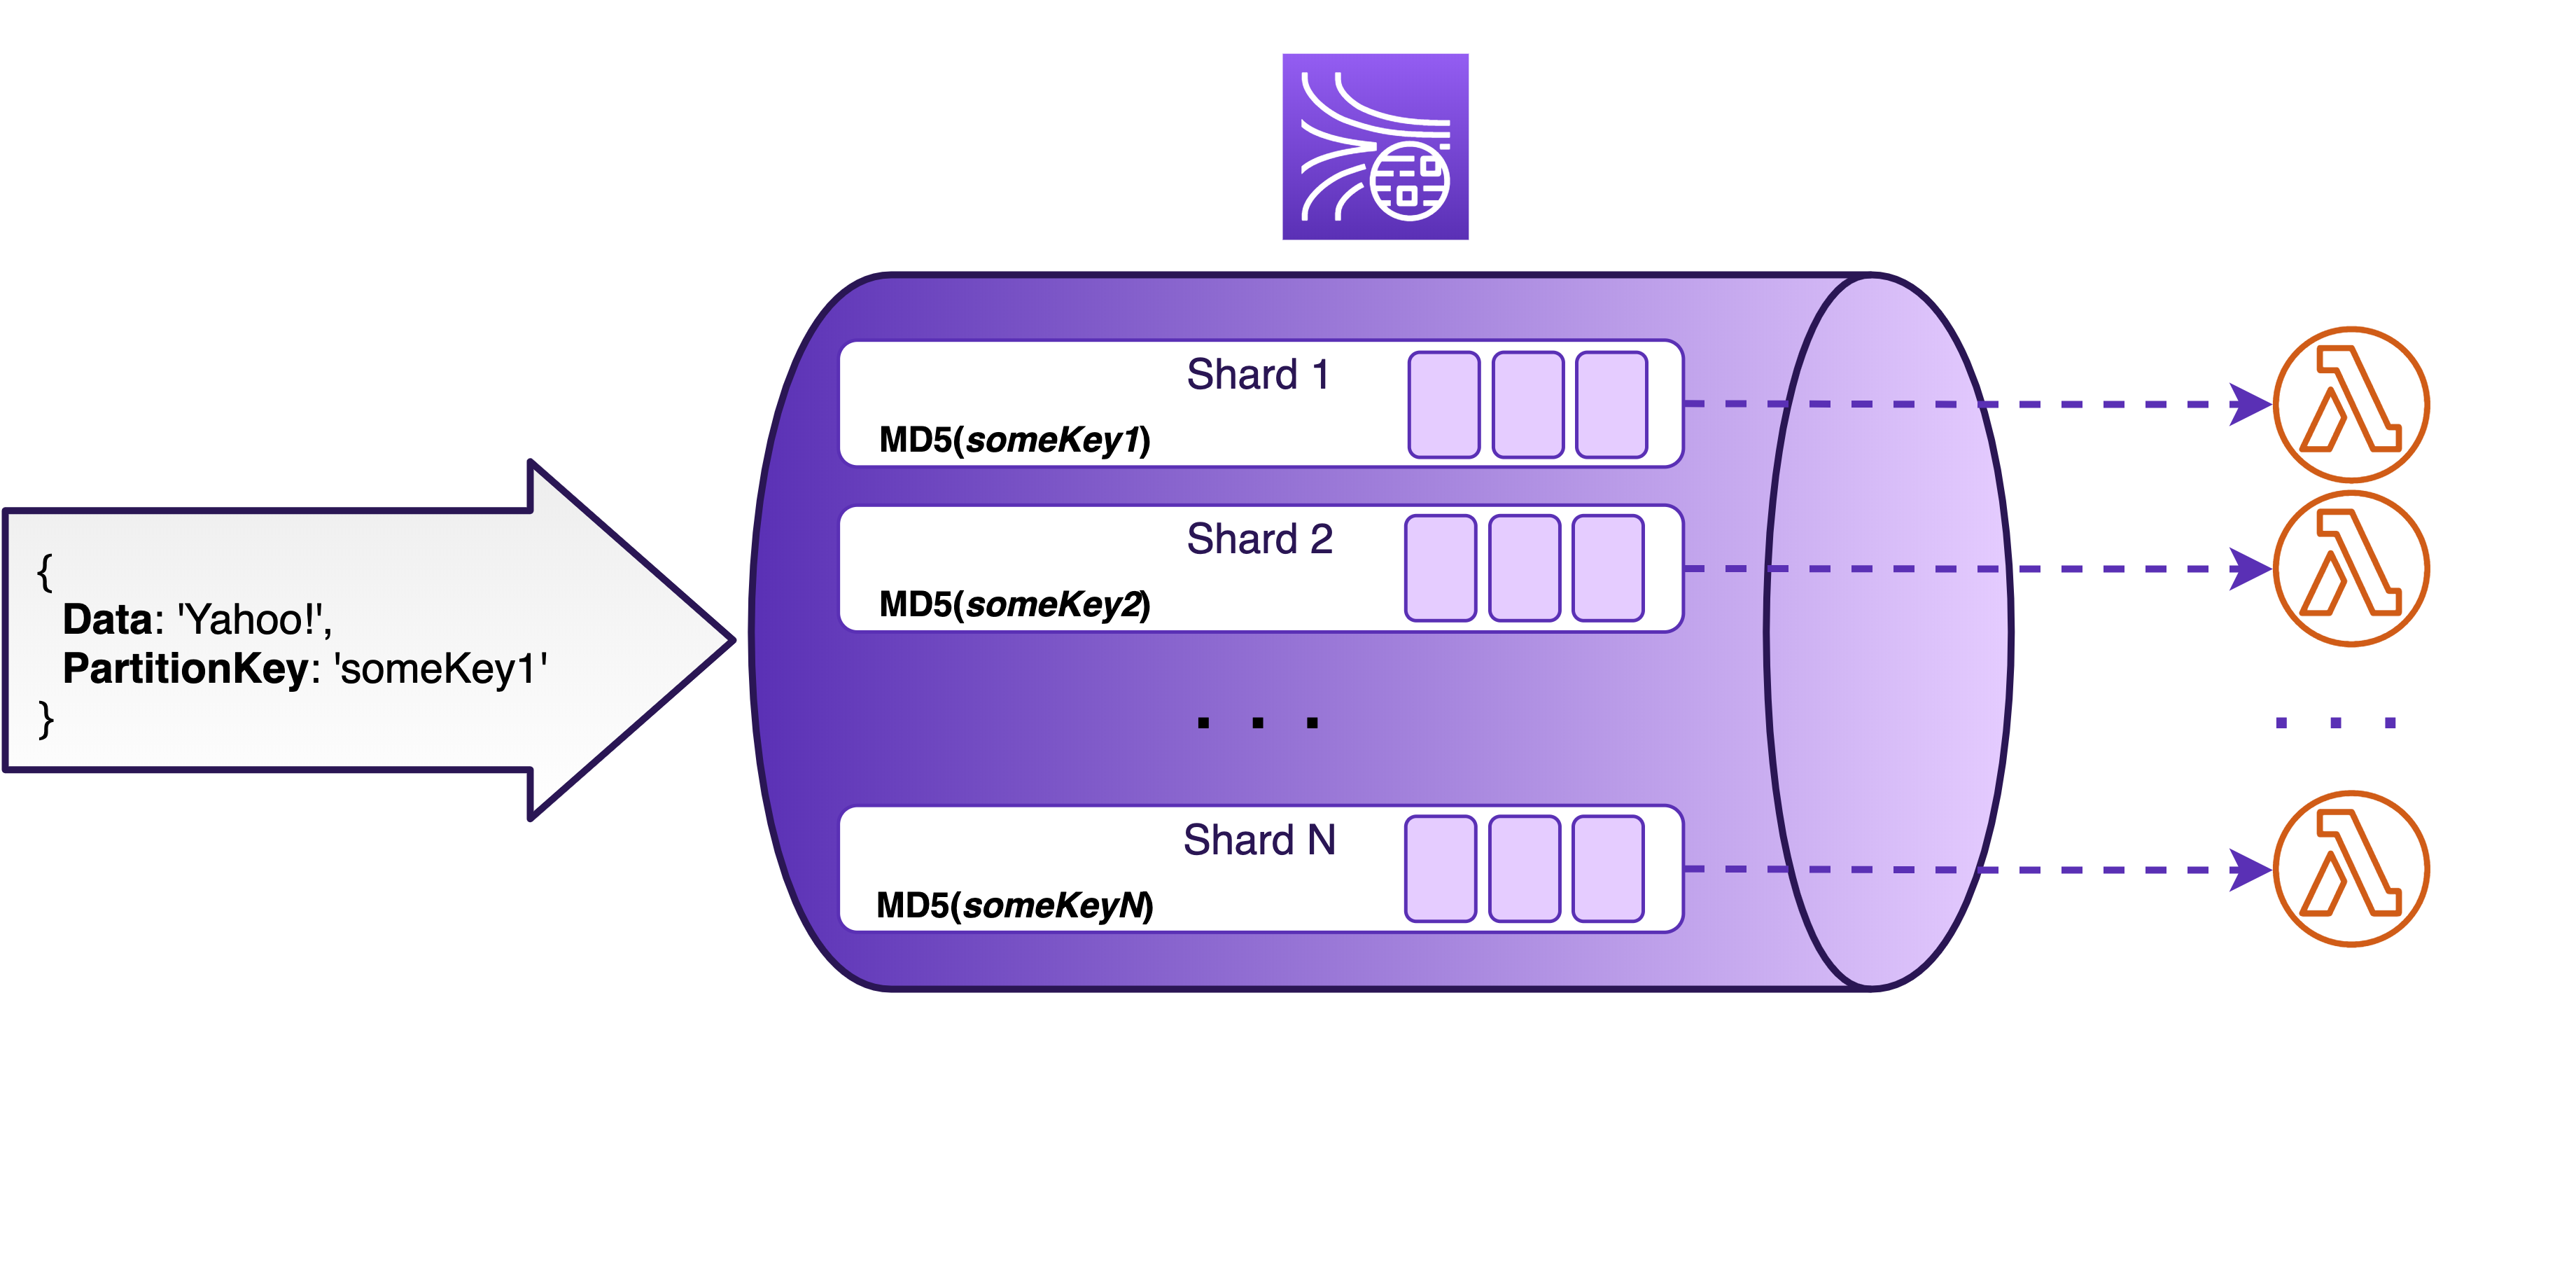
\includegraphics[width=\textwidth]{graphics/kinesis-inner-workings.png}
\caption[Funktionsweise von Kinesis]{Funktionsweise von Kinesis.\footnotemark}
\label{abb:KinesisShards}
\end{figure}
\footnotetext{Entnommen aus: \cite{Pogosova.28.05.2020}}
Kinesis unterteilt, wie in \autoref{abb:KinesisShards} gezeigt, Daten in einzelne Partitionen/Shards, in denen gleich partitionierte Datensätze verarbeitet werden können.\footcite[Vgl. auch im Folgenden][]{Pogosova.28.05.2020} Einzelne Shards verhalten sich dabei wie geordnete Warteschlangen und speichern die Nachrichten nach Eingangsdatum sortiert. 

\produktbewertung{Amazon~Kinesis}{11,5,4,4,6,6,5,0,3,2,0,46}
\autoref{tab:bewertungsmatrix-Amazon~Kinesis}

\subsection{AWS Lambda}
Bei \ac{AWS} Lambda handelt es sich um die Amazon Implementierung eines \ac{FaaS} Dienstes. Innerhalb dieser Arbeit wird Lambda als einzige generelle Computing Plattform betrachtet, da Alternativen wie \ac{EC2}, welches virtuelle Maschinen anbietet oder \ac{ECS}, welches Container anbietet einen von einzelnen Events unabhängigen Lebenszyklus haben. So laufen Container auf \ac{ECS} oder virtuelle Maschinen auf \ac{EC2}, wenn nicht anders konfiguriert kontinuierlich und holen/ \enquote{fetchen} Daten. In Zeiträumen, in denen keine Daten bereitstehen sind die entsprechenden Container und virtuellen Maschinen im Leerlauf, was unnötige Kosten erzeugt. Lambda hingegen wird von unterstützenden Diensten zur Verarbeitung von Events aufgerufen. Dabei ist je nach Dienst einstellbar, ob ein Aufruf pro Event stattfinden soll, oder Events zu einer konfigurierbaren Anzahl gruppiert werden und dann an Lambda übergeben werden. Lambda eignet sich besonders für analytische Workloads, seit der kürzlichen Addition von Intels \ac{AVX2}, einem speziellen CPU-Instruktionssatz, der die Verarbeitung von Vektorinstruktionen, wie sie beispielsweise beim Machine Learning oder in der Statistik vorkommen, beschleunigt.\footcite[Vgl.][]{Beswick.24.11.2020} Aufgrund der zentralen Rolle im Bereich Compute bei \ac{AWS}, können viele Dienste Events an Lambda senden. In \autoref{abb:GrobArchitekturLambda} sind als Integrationsbeispiele die \acp{MoM} \ac{IoT} Core, MQ und Kinesis Data Streams als Eventlieferanten gezeigt.
\begin{figure}[H]
\centering
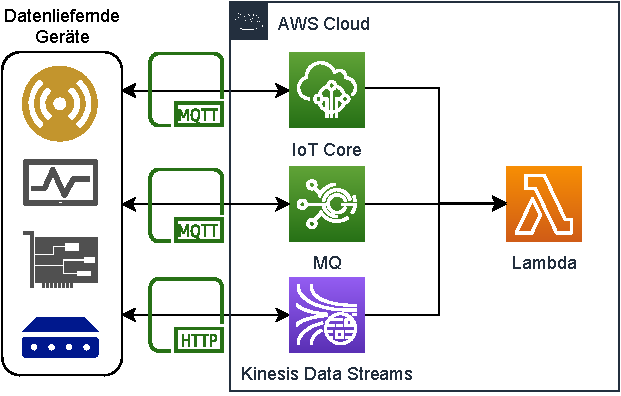
\includegraphics[width=0.8\textwidth]{graphics/Lambda-general.pdf}
\caption{Grobarchitektur des Ablaufes für Lambda}
\label{abb:GrobArchitekturLambda}
\end{figure}

\produktbewertung{AWS~Lambda}{8,10,9,6,7,6,0,0,3,2,1,52}
\autoref{tab:bewertungsmatrix-AWS~Lambda}

\subsection{Amazon MSK}
Bei \ac{MSK} handelt es sich um einen Managed Service für die Open Source Lösung Apache Kafka. Im Gegensatz zu anderen, hier im Kapitel aufgeführten Lösungen wie \ac{IoT} Analytics, hat Amazon \ac{MSK} nicht von Grund auf selber entwickelt, sondern einen großen Teil des Codes von Apache Kafka übernommen. Dies erklärt auch, warum die Anbindung an andere Dienste von Amazon bedeutend schwieriger ist, als beispielsweise an \ac{IoT} Core. In der in \autoref{abb:GrobArchitekturMSK} abgebildeten Grobarchitektur müsste zur Anbindung von Apache Kafka an zuliefernde Geräte ein Intermediär wie \ac{IoT} Core verrwendet werden, da Apache Kafka ein eigenes, binäres Protokoll hat, welches sonst in die Geräte implementiert werden müsste. \Todo{letzten Halbsatz belegen} Fraglich ist, ob sich eine Implementierung des Kafka Protokolls auf allen Endgeräten lohnt, speziell im Licht besser unterstützter Standards wie \ac{MQTT}. Umgangen werden kann die Implementierung des Kafka Protokolls auf zuliefernden Geräten auf dreierlei Arten: Zum einen lassen sich mittels Kafka Connect for \ac{MQTT} \ac{MQTT} Broker als Eventquellen anbinden.\footcite[Vgl.][]{Erber.12.01.2021} Alternativ kann Kafka auch als \ac{MQTT} Proxy dienen, was bedeutet, dass Kafka als eigenständiger MQTT Broker agiert, wobei zu beachten ist, dass Kafka weit nicht alle \ac{MQTT} Standardelemente implementiert und eine paralelle Weiterverarbeitung in anderen Amazon Diensten nicht möglich ist.\footcite[Vgl.][]{Erber.12.01.2021} Zuletzt gibt es noch die Möglichkeiten, die Nachrichten via \ac{IoT} Core innerhalb von \ac{AWS} an \ac{MSK} weiterzuleiten, was auch in \autoref{abb:GrobArchitekturMSK} dargestellt ist.
\begin{figure}[H]
\centering
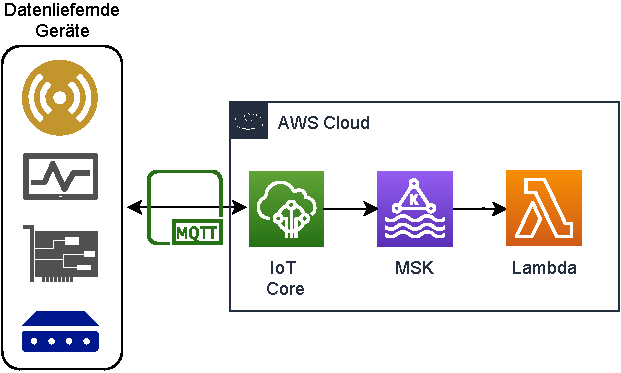
\includegraphics[width=0.8\textwidth]{graphics/MSK-general.pdf}
\caption{Grobarchitektur des Ablaufes für Managed Streaming for Apache Kafka}
\label{abb:GrobArchitekturMSK}
\end{figure}

Kafka hat eigene Verarbeitungslogiken integriert, mit welchen einige Analysen bereits durchgeführt werden können. Um diese in \ac{AWS} weiterverarbeiten zu können, müssen die Ergebnisse via der Integration mit Lambda oder der Integration mit \ac{EC2}, der Amazon Plattform für virtuelle Maschinen abgerufen werden.

\produktbewertung{Amazon~MSK}{11,5,4,7,5,6,5,0,3,1,1,48}
\autoref{tab:bewertungsmatrix-Amazon~MSK}

% => binary protocol no \ac{MQTT} Support, redundant, only Lambda and EC2 conenctivity

\subsection{AWS Glue}
Mittels dem \ac{AWS} Glue Dienst, welcher diverse \ac{ETL} Dienste, wie beispielsweise Datenkatalogisierung und Datentransformation basierend auf dem Apache Spark Ökosystem anbietet, können ebenfalls Streams analysiert werden.\footcite[Vgl.][]{AmazonWebServicesInc..o.J.d}\nzitat\footcite[Vgl. auch im Folgenden][]{AmazonWebServicesInc..2020} Basierend auf der Apache Spark Structured 
Streaming-Engine können nach Aussage des Herstellers Daten aus Kinesis oder Kafka (und damit aus \ac{MSK}) geladen werden. Nachfolgend werden die eingehenden Daten mittels sogenannter Jobs analysiert/transformiert, welche in Sprachen wie Scala, Java, Python oder R geschrieben sein können. Nach Abschluss der Analyse können die Daten in \ac{S3} oder in eine \ac{JDBC} kompatible Datenbank (z.B. MySQL, PostgreSQL, Amazon Redshift, Oracle Databse, ...) geladen werden.\footcite[Vgl.][]{AmazonWebServicesInc..o.J.e} Die Interaktion zwischen eigener Logik und AWS Glue erfolgt via \acp{API} von Apache Spark, die entsprechende Kentnisse zur Interaktion mit den Daten erfordern.

\produktbewertung{AWS~Glue}{8,10,9,6,4,4,5,0,2,1,0,49}
\autoref{tab:bewertungsmatrix-AWS~Glue}

\subsection{Produktauswahl}

\begin{table}[H]
\centering
\begin{tabular}{|l|l|l|}
\hline
Platz & Name & Summe \\ \hline
1 & AWS Lambda & \cellcolor[HTML]{DAE8FC}52 \\ \hline
2 & AWS Glue & \cellcolor[HTML]{DAE8FC}49 \\ \hline
3 & Amazon MSK & \cellcolor[HTML]{DAE8FC}48 \\ \hline
4 & AWS IoT Events & \cellcolor[HTML]{DAE8FC}47 \\ \hline
5 & Amazon Kinesis & \cellcolor[HTML]{DAE8FC}46 \\ \hline
\end{tabular}
\caption{Produktreihenfolge Echtzeitprodukte}
\label{tab:Reihenfolge-Echtzeit}
\end{table}
